\documentclass[12pt,twocolumn]{IEEEtran}

\usepackage[utf8]{inputenc}
\usepackage{xcolor}
\usepackage{fontenc}
\usepackage{graphicx}
\usepackage{float}
\usepackage[dvips]{hyperref}
\title{I$^{2}$C Protocol}
\author{\IEEEauthorblockN{Varanasi Shashank}
\IEEEauthorblockA{- ES16BTECH11025\\}
\and
\IEEEauthorblockN{Akshita Ramya}
\IEEEauthorblockA{- ES16BTECH11012\\}
\and
\IEEEauthorblockN{Aravind Ganesh}
\IEEEauthorblockA{- EE16BTECH11026\\}
\and
\IEEEauthorblockN{Srinidhi Bachu}
\IEEEauthorblockA{- ES16BTECH11029\\} 
\and
\IEEEauthorblockN{Jeel Bhavsar}
\IEEEauthorblockA{- ES16BTECH11005} 
}

\date{02/05/2017}
 
\begin{document}
  \maketitle
    \section{Introduction}
    
     Embedded electronics is all about interlinking circuits (processors or other integrated circuits) to create a symbiotic system. In order for those individual circuits to swap their information, they must share a common communication protocol. Hundreds of communication protocols have been defined to achieve this data exchange, and, in general, each can be separated into one of two categories: parallel or serial.

In computer architecture, a bus is a communication system that transfers data between components inside a computer, or between computers. This expression covers all related hardware components (wire, optical fiber, etc.) and software, including communication protocols.

   \subsection {Serial communication}

In telecommunication and data transmission, serial communication is the process of sending data one bit at a time, sequentially, over a communication channel or computer bus. This is in contrast to parallel communication, where several bits are sent as a whole, on a link with several parallel channels.

Serial communication is used for all long-haul communication and most computer networks, where the cost of cable and synchronization difficulties make parallel communication impractical. Serial computer buses are becoming more common even at shorter distances, as improved signal integrity and transmission speeds in newer serial technologies have begun to outweigh the parallel bus' advantage of simplicity and to outstrip its disadvantages.

Integrated circuits are more expensive when they have more pins. To reduce the number of pins in a package, many ICs use a serial bus to transfer data when speed is not important. Some examples of such low-cost serial buses include SPI, I$^{2}$C, dc-bus, UNI/O, and 1-Wire.

  
    \section{The physical I$^{2}$C bus}
    I$^{2}$C (Inter-Integrated Circuit),  is a multi-master, multi-slave, packet switched, single-ended, serial computer bus invented by Phillips Semiconductor. It is typically used for attaching lower-speed peripheral ICs to processors and micro-controllers in short-distance, intra-board communication. I$^{2}$C is appropriate for peripherals where simplicity and low manufacturing cost are more important than speed. \newline SCL is the clock line. It is used to synchronize all data transfers over the I$^{2}$C bus. SDA is the data line. The SCL and SDA lines are connected to all devices on the I$^{2}$C bus.

  \subsection{Masters and Slaves}
      The devices on the I$^{2}$C bus are either masters or slaves. The master is always the device that drives the SCL clock line. The slaves are the devices that 
      respond to the master. There can be, and usually are, multiple slaves on the I$^{2}$C bus. Slaves will never initiate a transfer. Both master and slave can transfer 
      data over the I$^{2}$C bus, but that transfer is always controlled by the master.
  
  \section{The I$^{2}$C Physical Protocol}

    Data is transferred in sequences of 8 bits. The bits are placed on the SDA line starting with the MSB (Most Significant Bit). The SCL line is then pulsed high, then low. For every 8 bits transferred, the slave receiving the data sends back an acknowledge bit, so there are actually 9 SCL clock pulses to transfer each byte of data. If the slave sends back a low ACK bit, then it has received the data and is ready to accept another byte. If a high is sent, then it indicates no further data can be accepted. 
    \newline
A start sequence is one of two special sequences defined for the I$^{2}$C bus, the other being the stop sequence. The start sequence and stop sequence are special in that these are the only places where the SDA (data line) is allowed to change while the SCL (clock line) is high. When data is being transferred, SDA must remain stable and not change whilst SCL is high. The start and stop sequences mark the beginning and end of a transaction with the slave device.

  \begin{figure}[H]
    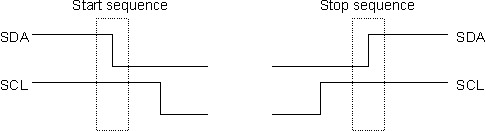
\includegraphics[width=\linewidth]{start_stop_seq.jpeg}
    \caption{}
  \end{figure}




    \subsection{I$^{2}$C Device Addressing}
	Here, the I$^{2}$C address has 7 bits. When sending out the 7 bit address, we still always send 8 bits. The extra bit indicates if the master is writing to or reading from the slave. If the R/W bit is '0' the master is writing to the slave. If the bit is '1', the master is reading from the slave. The 7 bit address is placed in the upper 7 bits of the byte and the Read/Write (R/W) bit is the LSB (Least Significant Bit).
	
    \begin{figure}[H]
	  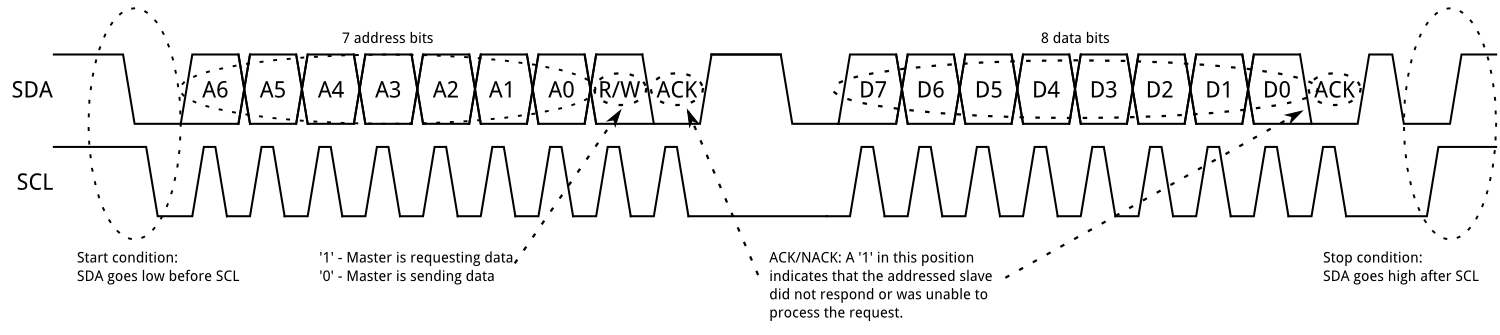
\includegraphics[width=\textwidth]{i2c_concept.png}
	  \caption{The I$^{2}$C protocol}
     \end{figure}


  \section{Theory of Operation}
    \begin{description}
     
     \item[$\bullet$] The I$^{2}$C master we implemented uses the state machine depicted in Figure 3 to implement the I$^{2}$C-bus protocol. Upon start-up, the component immediately enters the ready state(here, enters and remains in idle state till an edge trigger happens). 

     \item[$\bullet$] Once an edge trigger happens the start state generates the start condition on the I$^{2}$C bus, and the command state communicates the address(start\_addr\_tx) and rw command to the bus. 

    \item[$\bullet$] The slv\_ack1 state(slave\_hit\_addr) then captures and verifies the slave’s acknowledgment(ack\_one), if not acknowledged goes back to idle state. 

    \item[$\bullet$]Depending on the rw command, the component then proceeds to either write data to the slave (wr state) or receive data from the slave (rd state). 
    In our implementation, we have dealt with write only. If it hits read, it goes back to idle state.

    \item[$\bullet$] Once state\_reg hits write, it will keep receiving bits of data to write to slave till bit\_cnt reaches 7 (8 bits of data sent).

    \item[$\bullet$] Once bit\_cnt equals 8, depending on the acknowledgment we receive from slave\_hit\_data , the state either ends the process (ack\_two =0) or goes back 
    to idle state(ack\_two =1). 

    \item[$\bullet$] Once the process has finished running successfully (i.e. ack\_two =0) it goes back to idle state and waits for the edge trigger (sda). If sda is received 
    as 1, then our I$^{2}$C repeats the process over again from start.
    \end{description}
  
    \begin{figure}[p]
    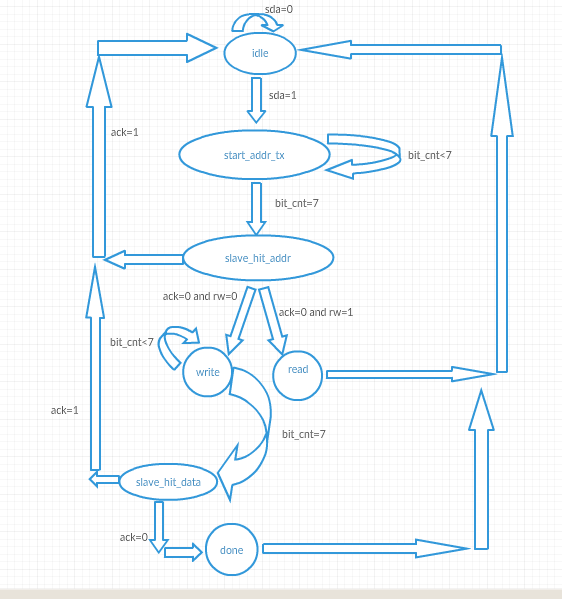
\includegraphics[width=1.6\linewidth, height=20cm]{I2C_State_diagram.png}
    \caption{State Diagram}
    \end{figure}

\end{document}


